%!TEX TS-program = xelatex
%!TEX root = ../../maxwell2018thesis.tex

\chapter[Result Diversification and Stopping Behaviour]{Result Diversification and\\Stopping Behaviour}\label{chap:diversity}
A searcher, when developing an information need, will often possess an incomplete mental model of the topic. As such, they may arrive at a retrieval system with an \emph{Anomalous State of Knowledge (ASK)}~\citep{belkin1980ask}. To address this deficiency in their mental model, a searcher will often issue a variety of different queries to explore the topic space~\citep{kelly2015search_tasks}. Often, such topics are \emph{aspectual} in nature, where an underlying goal is to find out about the different facets, dimensions or aspects\footnote{We consider aspects in this chapter, defined as `\emph{`roughly one of many possible answers to a question which the topic in effect poses''}~\citep{over1998trec}.} of the topic. An example of aspects within a topic is illustrated below, taken from TREC Robust Track~\citep{voorhees2006trec_robust} topic 347.

\begin{figure}[h]
    \centering
    \vspace{4mm}
    \resizebox{1\hsize}{!}{
    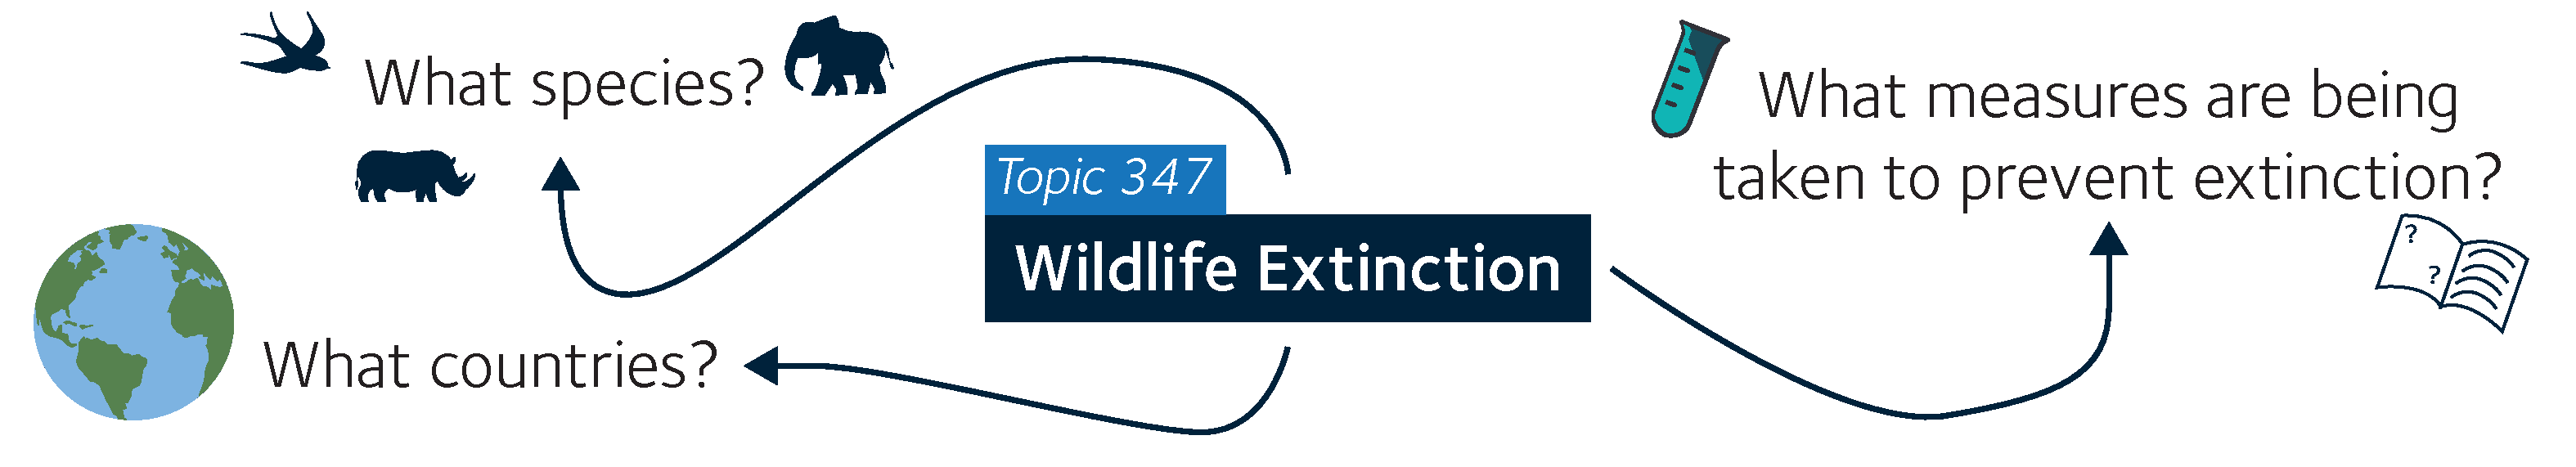
\includegraphics{figures/ch8-aspects_intro.pdf}}
    \label{fig:aspectsintro}
    \vspace{-5mm}
\end{figure}

While \emph{aspectual retrieval} has been heavily studied in the past (most prominently during the \emph{\gls{acr:trec} Interactive Tracks}~\citep{over2001trec}), there has been renewed interest in this type of search task. This is because it represents a novel context to explore the idea of \emph{``searching as learning''}~\citep{collins2017sal}. In this context, the goal of the system is to help the searcher learn about a topic~\citep{collins2017sal} -- and in doing so, the number of aspects the searcher finds provides an indication of how much they learned during the process~\citep{syed2017sal}. If the goal is to help searchers learn about a topic, then by returning results that are more diverse in nature and presenting a broader view of the topic, this \emph{should} assist searchers learn more about said topic. This reasoning suggests that employing \emph{diversification} will lead to an improved search and learning experience~\citep{syed2017sal}.

However, while there have been numerous diversification algorithms developed and proposed over the years\footnote{There are numerous examples of work on search result diversification, including measures such as \emph{Maximal Marginal Relevance (MMR)}~\citep{carbonell1998mmr}, and the \emph{xQuAD} framework~\citep{santos2010query_reformulations_diversification, santos2011intent}. Other studies in this area include works by~\cite{chen2006probabilistic_models} and~\cite{zhai2015subtopics}.}, the focus of the work reported in this chapter is on addressing the problem of intents, rather than how diversification affects complex search tasks, such as ad-hoc or aspectual retrieval. Thus, this chapter reports on:

\begin{itemize}
    \item{a user study, exploring how diversifying results (or not) affects the search behaviour and performance of searchers when undertaking different search tasks, from one of ad-hoc or aspectual retrieval (Section~\ref{sec:diversity:users}); and}
    \item{a simulated study, examining the various stopping strategies proposed in Chapter~\ref{chap:strategies}, utilising the~\gls{acr:csm}, perform under these tasks (Section~\ref{sec:diversity:simulated}).}
\end{itemize}

In particular, we use~\glsfirst{acr:ift}~\citep{pirolli1999ift} in this chapter -- outlined in Section~\ref{sec:stopping_background:models:theoretical:ift} on page~\pageref{sec:stopping_background:models:theoretical:ift} -- to derive a number of hypotheses, and thus ground our work. We begin this chapter however with a discussion of the prior work in the area, focusing upon aspectual retrieval, and a brief discussion of how~\gls{acr:ift} is used to provide us with a series of hypotheses about searcher behaviours across the different experimental conditions we trial.

\section{Background, Motivation and Hypotheses}\label{sec:diversity:background}
As discussed previously, a searcher will likely pose a varying number of queries (and~\glsplural{acr:serp}), and examine a number of documents (if any) before issuing a new query, or stopping their search altogether. The reasons for stopping are numerous. Stopping at a \emph{session level} can occur because:

\begin{itemize}
    \item{they have simply found enough information~\citep{prabha2007enough, dostert2009satisficing, hassan2013beyond_clicks};}
    \item{have run out of time~\citep{zach2005enough_is_enough}; or}
    \item{were dissatisfied with what they found~\citep{kiseleva2015serp_fails}; or}
    \item{simply gave up their search~\citep{diriye2012abandonment}.}
\end{itemize}

Numerous works have shown that different factors influence search behaviours -- this is demonstrated in Chapter~\ref{chap:snippets}, for instance, which showed how varying the length of result summaries influences behaviours. However, of particular relevance to this chapter is how different \emph{search tasks} influence a searcher's behaviours~\citep{kelly2015search_tasks}.

\subsection{Aspectual Retrieval}
An interesting search task that has not received much attention as of late is \emph{aspectual retrieval.} Aspectual retrieval is a type of search task that concerns the identification of different \emph{aspects} of a given topic. This task type differs from traditional ad-hoc retrieval in the sense that ad-hoc retrieval is concerned only with what constitutes a \emph{relevant} document to a given topic, rather than identifying relevant documents, and whether they are \emph{different} to what has been previously observed.

A relevant and different document will contain unseen aspects associated with the topic in question. With a graphical example provided at the beginning of this chapter, we now provide a further example to aid understanding. Consider the topic \emph{wildlife extinction} from the~\gls{acr:trec} 2005 Robust Track~\citep{voorhees2006trec_robust}. In an ad-hoc search task, if the searcher manages to find several documents concerning \texttt{Pandas in China}, these would all be considered relevant. However, for an aspectual retrieval task, where \emph{different} aspects must be found, the first document concerning \texttt{Pandas in China} is considered to be relevant/useful, and other aspects (in this case, the species of endangered animal) would need to be found, such as \texttt{Sumatran Rhinos in Malaysia}, \texttt{Crested Ibis in Japan}, etc.

Aspectual retrieval found significant traction in the \emph{\gls{acr:trec} Interactive Tracks}~\citep{over2001trec} from 1997-2002. The overarching goal of these tracks was to investigate searching, and an interactive task, by examining the processes involved, as well as the outcome~\citep{over2001trec}. Interaction was considered from the inaugural \emph{\gls{acr:trec}-1} in 1993~\citep{harman1993trec1}, where one group investigated interactive searching under the so-called \emph{interactive query mode} while undertaking an ad-hoc task. From \emph{\gls{acr:trec}-6} (1997) to \emph{\gls{acr:trec} 2002}, a substantial volume of research was directed towards the development of systems and search interfaces that:

\begin{itemize}
    \item{assisted searchers in exploring and retrieval various aspects of a topic, such as cluster-based and faceted interfaces that explicitly showed different aspects~\citep{mcdonald1998interactive, villa2009aspect_interface};}
    \item{provided tiles and stacks to organise documents~\citep{hearst1995tilebars, hearst1997texttiling, harper2006piling, iwata2012tilediversified}; and}
    \item{provided mechanisms to provide query suggestions that led to subjects following different search paths~\citep{kato2012query_suggestion, umemoto2016scentbar}.}
\end{itemize}

However, a disappointing conclusion from this initiative was that little difference was observed between such systems and the standard control systems (i.e. the traditional \emph{ten blue links}, as previously discussed in this thesis) -- both in terms of behaviour and performance~\citep{voorhees2005trec_book}.

As work shifted from aspectual retrieval to other areas, studies related to determining the intent of a searcher's query began to take hold, where the goal of this problem is to diversify the results retrieved with respect to the original query~\citep{rose2004understanding_user_goals}. Thus, this addresses the problem of \emph{ambiguity} for short, impoverished queries. This led to a series of diversification algorithms (and intent-aware evaluation measures), changing focus from the interface to the underlying algorithms and their evaluation measures. However, while there have been numerous studies investigating the effectiveness of diversification algorithms for the problem of query intents (e.g. one query, several possible interpretations), little work has looked at studying how such algorithms apply in the context of aspectual retrieval (e.g. one topic, many aspects). This is many due to the fact that most of these algorithms were developed \emph{after} the~\gls{acr:trec} Interactive Track finished in 2002.

Recently however, a growing interest in new, more complex and exploratory search tasks has taken hold. This is true in the aforementioned context of \emph{``searching as learning''}~\citep{collins2017sal}.~\cite{syed2017sal} hypothesised that diversifying the results presented to searchers would improve their learning efficiency, and that this would be observed by a change in vocabulary expressed in their queries. This work reported in this chapter motivates our interest examining the effects of diversification when considering the task of aspectual retrieval, where a searcher needs to learn about different aspects of a topic. To ground our work, we now consider how search behaviours are likely to be changed by generating a series of hypotheses from~\gls{acr:ift}.

\subsection{Tasks and Information Foraging Theory}\label{sec:diversity:background:tasks}
To motivate our hypotheses for this chapter, we can draw upon~\gls{acr:ift}~\citep{pirolli1999ift}, and the \emph{patch model} in particular, to ground our research and provide insights into how search behaviours may change. The patch model, as detailed in Section~\ref{sec:stopping_background:models:theoretical:ift}, provides a mechanism for predicting how long foragers will stay in a patch before moving onwards to the next. Using the established approach discussed previously -- where moving between patches is akin to issuing a new query, while staying within a patch considered examining a~\gls{acr:serp} and linked documents -- we can then make a series of predictions as to how searchers will behave under different experimental conditions.

\begin{figure}[t!]
    \centering
    \resizebox{1\hsize}{!}{
    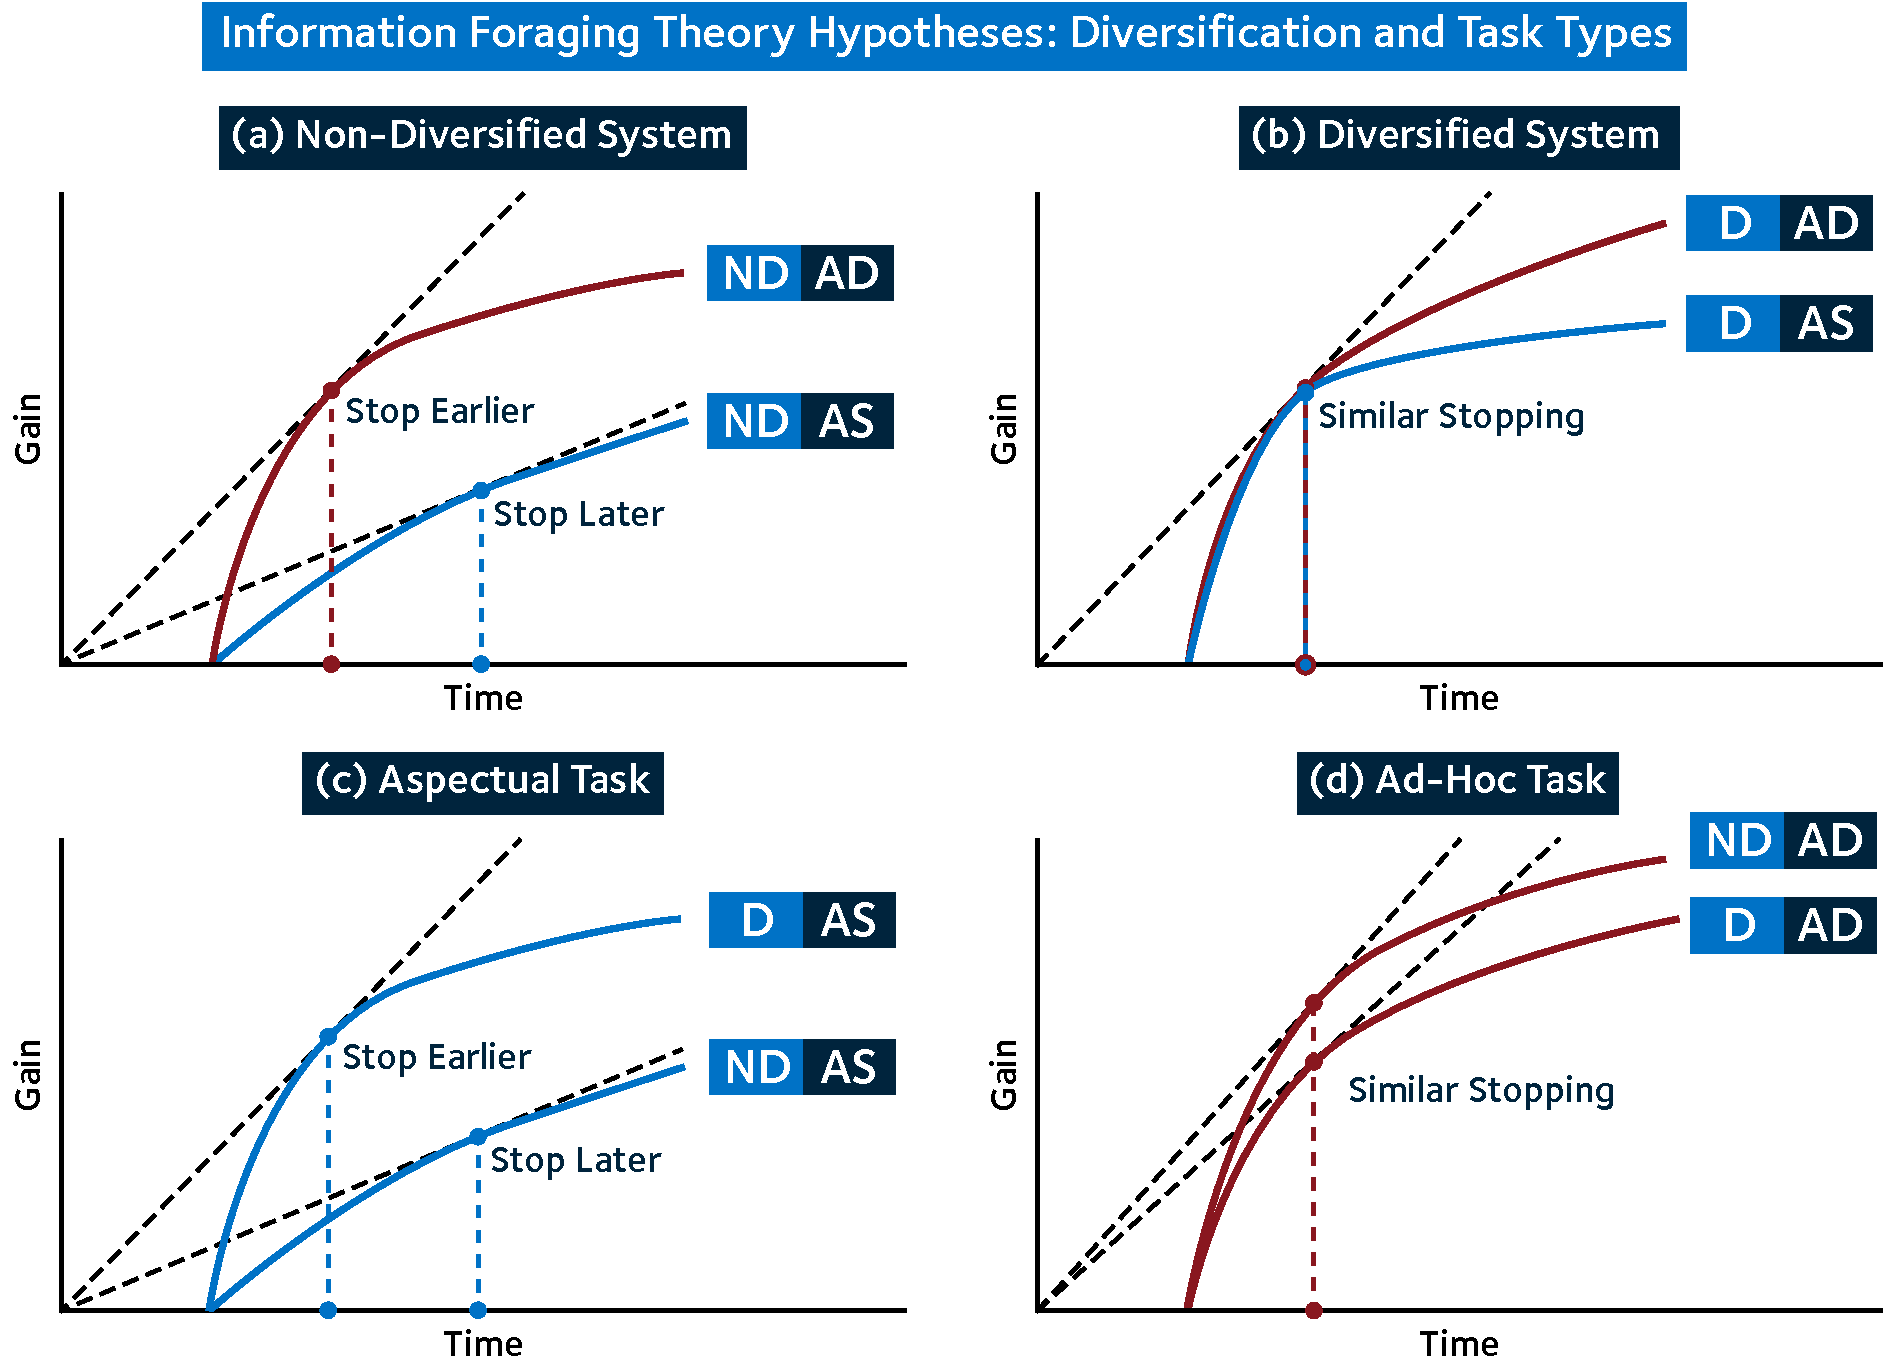
\includegraphics{figures/ch8-ift_theory_plots.pdf}}
    \caption[\gls{acr:ift} and Diversification: Hypothesis Illustrations]{Graphical illustrations of the hypotheses motivated by~\gls{acr:ift}, with each plot showing how stopping behaviour is likely to be affected when using a system that \emph{(a)} diversifies results and \emph{(b)} doesn't, and over \emph{(c)} aspectual and \emph{(d)} ad-hoc tasks. Section~\ref{sec:diversity:users:method} enumerates the four different experimental conditions shown here, such as \dualbluebox{ND}{AD} for instance.}
    \label{fig:ift_theory}
\end{figure}

These predictions are graphically illustrated in the four plots shown in Figure~\ref{fig:ift_theory} -- over a diversified \blueboxbold{D} and non-diversified \blueboxbold{ND} system, with ad-hoc \darkblueboxbold{AD} and aspectual \darkblueboxbold{AS} retrieval tasks.\footnote{The system and task are combined together to produce a complete condition, such as \dualbluebox{ND}{AD} representing a non-diversified system, with an ad-hoc retrieval task.} Gain curves for each of the four conditions are shown. In the top left plot~\ref{fig:ift_theory} \emph{(a)}, where a non-diversified system is being used, the gain curve for the ad-hoc retrieval task is higher, as any relevant document contributes to the searcher's gain. Conversely, the gain curve is lower for the aspectual retrieval task. This is because similar relevant documents would not contribute to the overall level of gain experienced by the searcher.

From~\gls{acr:ift}, the optimal stopping point would be different between the two tasks. As we discussed in~\ref{sec:stopping_background:models:theoretical:ift}, we can graphically find this point by drawing a line from the origin to the tangent of the gain curve. Red and blue dots indicate the optimal stopping points for ad-hoc and aspectual retrieval, respectively.~\gls{acr:ift} therefore suggests that with a non-diversified system, searchers will examine more documents per query for aspectual retrieval tasks when compared to ad-hoc tasks.
Discuss IFT, and then lead onto the hypotheses.

Plot~\ref{fig:ift_theory} \emph{(b)} illustrates gain curves where a diversified system would be used, with gain curves for ad-hoc and aspectual retrieval being similar in nature. This is because the diversified should bring relevant but different documents closer to the top of the rankings earlier. In the case of ad-hoc retrieval, these relevant (even if different) documents would still contribute to the overall level of gain. For aspectual retrieval, relevant and different documents will also contribute to the overall level of gain experienced by the searchers -- up to the point where the documents become similar to previously examined material. Therefore,~\gls{acr:ift} appears to suggest that similar stopping behaviours would be observed when searchers use a diversified search system.

Plot~\ref{fig:ift_theory} \emph{(c)} shows the predicted stopping behaviour for the aspectual retrieval task, where we have plotted the aspectual gain curves from the system plots \emph{(a)} and \emph{(b).} Interestingly,~\gls{acr:ift} suggests that searchers will stop sooner when using the diversified system. As such, if searching for the same length of time, searchers would thus issue more queries. Finally plot~\ref{fig:ift_theory} \emph{(d)} shows the predicted stopping behaviour for the ad-hoc retrieval task, where again we plot the curves from the respective systems in plots \emph{(a)} and \emph{(b).} Note that here, the gain curve for the diversified system may be a little lower as some irrelevant but different material may bubble up the rankings. However, as can be seen, we expect little difference overall between the two systems, and so we hypothesise that the two levels of gain (and searcher behaviours) will be approximately be the same. Consequently,~\gls{acr:ift} suggests that there will be little difference in terms of stopping behaviours between the two systems with ad-hoc retrieval tasks.

However, we found~\gls{acr:ift} to counter our intuitions as to how searchers would \emph{behave.} When using a standard, non-diversified retrieval system, our intuition suggests that since the aspectual retrieval task is rather exploratory, searchers are then more likely to issue more queries as they learn about the topic, and try to explore efforts made by different countries to protect different specifies, for example.~\cite{kelly2015search_tasks} for example showed that more complex search tasks required a greater number of queries. If a searcher submits a query that retrieves relevant material such as \texttt{protecting Pandas in China}, then one would expect them to only select one or two examples, rather than many more. In the case of ad-hoc topic retrieval, we would \emph{intuitively} expected that searchers would issue fewer queries and examine more documents. This is because they don't need to find multiple aspects. However, when using a diversified system, which attempts to promote different aspects of a given topic, we would \emph{intuitively} expect that the behaviour of searchers would change, such that when undertaking aspectual retrieval, they would issue fewer queries and examine a greater number of documents per query.

\subsubsection{Hypotheses}\label{sec:diversity:background:tasks:hypotheses}
From the plots and descriptions provided above, we can formulate a number of different hypotheses relating to the expected searcher behaviours under different contexts.

Under aspectual retrieval search tasks, using a diversified system will lead to:
\begin{itemize}
    \item{\blueboxbold{H1} fewer documents examined per query; and}
    \item{\blueboxbold{H2a} more queries issued; or}
    \item{\blueboxbold{H2b} a decrease in the task completion time.}
\end{itemize}

With ad-hoc retrieval tasks, diversification will lead to:
\begin{itemize}
    \item{\blueboxbold{H3} no difference in the number of documents examined; and}
    \item{\blueboxbold{H4} no difference in the number of queries issued.}
\end{itemize}

While the contradiction between~\gls{acr:ift} and our intuitions provides an ulterior hypothesis. In addition, given the findings demonstrated by~\cite{syed2017sal}, we also hypothesis that diversification will lead to a greater awareness of the topic, regardless of the task put forward, as more aspects will be encountered and found.

\section{Diversifying Search Results}\label{sec:diversity:users}
Following on from the motivation and experimental,~\gls{acr:ift}-based hypotheses outlined above, this section discusses the user study that was undertaken in order to examine the aforementioned hypotheses. As per our general user study methodology discussed previously in Section~\ref{sec:method:user_study}, we conducted a within-subjects experiment, with the specific details for this study discussed in Section~\ref{sec:diversity:users:method} below.

The primary research question for this user study is as follows.

\begin{itemize}
    \item{\blueboxbold{RQ} How does diversification affect the search performance and behaviour when searchers under ad-hoc and aspectual retrieval tasks?}
\end{itemize}

This research question is addressed in tandem with the hypotheses put forward above in Section~\ref{sec:diversity:background:tasks:hypotheses}. Below, we now discuss the specific details for this user study, before discussing the results, with an emphasis on stopping behaviours, and whether or not the empirical evidence supports our hypotheses.

\subsection{Methodology}\label{sec:diversity:users:method}
As discussed above, this section outlines the specific details of this user study, and is to be considered in conjunction with the general user study methodology we employ, outlined in Section~\ref{sec:method:user_study}. The same basic retrieval system employing BM25, document corpus and topics were used as previously discussed.

The within-subjects study considers two key factors: the \emph{system} and the \emph{task.} For the system factor, our baseline control system was based upon BM25 (i.e. no diversification), and a diversified system. The details of our diversification approach are discussed in Section~\ref{sec:diversity:users:diversifying}. For the task factor, we used the standard ad-hoc retrieval task, and compared this against the aspectual retrieval task. This resulted in a $2x2$ factorial design. Each subject who took part in this study therefore completed four different search tasks, one in each of the four conditions (as we enumerate below). Each of the conditions were assigned using a Latin square rotation to minimise any ordering effects. The conditions listed below are also used in Section~\ref{sec:diversity:background:tasks} when explaining the plots supporting our hypotheses.

The first two conditions consider a non-diversified retrieval system \blueboxbold{ND} (i.e. BM25, our baseline).

\begin{itemize}
    \item{\dualbluebox{ND}{AS} A non-diversified system, with an aspectual retrieval task.}
    \item{\dualbluebox{ND}{AD} A non-diversified system, with an ad-hoc retrieval task.}
\end{itemize}

Our second set of conditions therefore consider a diversified system \blueboxbold{D}, using BM25 as a baseline and an additional diversifying component, as we discuss later in Section~\ref{sec:diversity:users:diversifying}.

\begin{itemize}
    \item{\dualbluebox{D}{AS} A diversified system, with an aspectual retrieval task.}
    \item{\dualbluebox{D}{AD} A diversified system, with an ad-hoc retrieval task.}
\end{itemize}

With non-diversifying and diversifying systems, we developed different sets of branding for each system, each with their own distinct colour scheme, name and logo. This was to assist searchers in differentiating between the two. First, in terms of branding, we created two fictional search engine names:

\begin{itemize}
    \item{\blueboxbold{YoYo Search}, representing the non-diversified \blueboxbold{ND} system; and}
    \item{\blueboxbold{Hula Search}, representing the diversified \blueboxbold{D} system.}
\end{itemize}

\begin{figure}[t!]
    \centering
    \resizebox{1\hsize}{!}{
    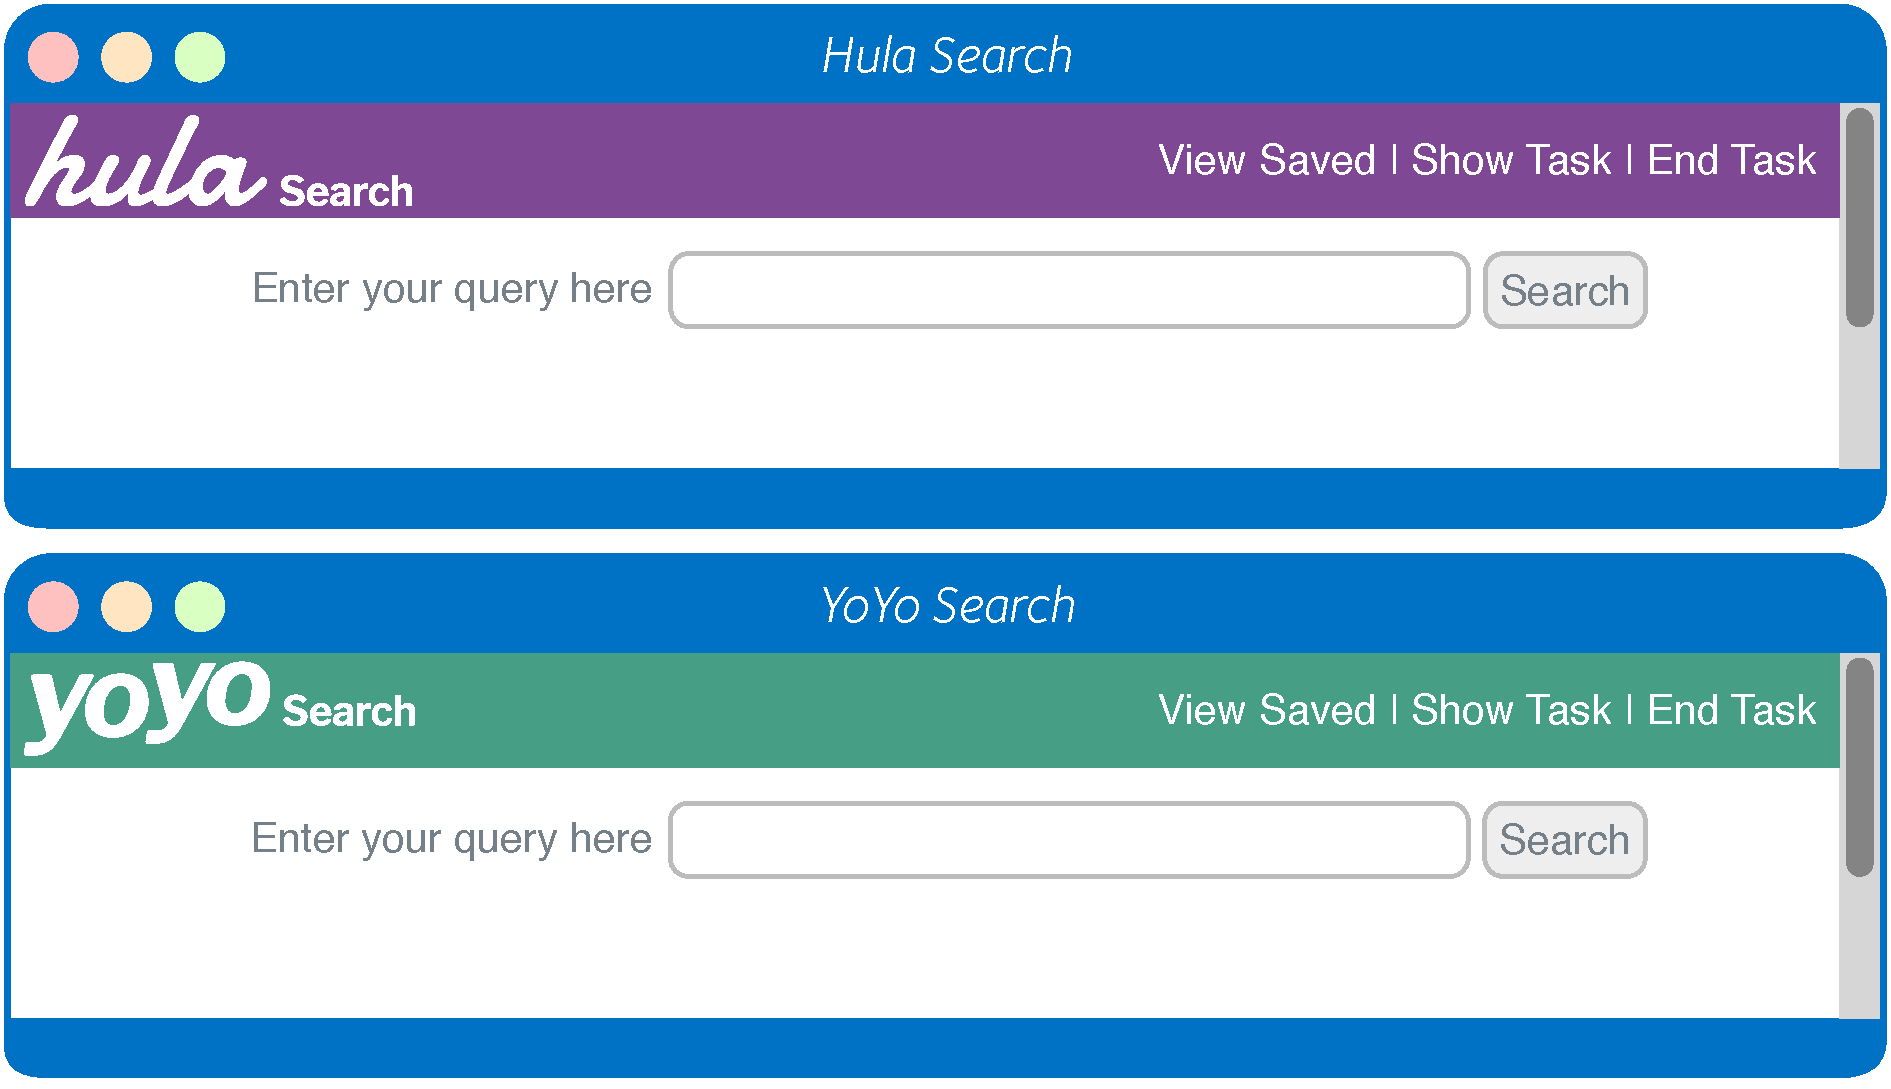
\includegraphics{figures/ch8-interface_headers.pdf}}
    \caption[Diversity user study interface mockups]{Mockups of the two names and colour schemes used to differentiate between the two experimental systems used in this user study. \emph{Hula Search} and \emph{YoYo Search} represented the non-diversified and diversified systems respectively. Refer to Section~\ref{sec:diversity:users:method} for more information.}
    \label{fig:interface_headers}
\end{figure}

These names were chosen as they were not associated with any major search engine (to the best of our knowledge), nor did they imply that one of the systems performed better than the other. Colour schemes were chosen to provide the greatest different in visual appearance to those with colourblindness.\footnote{Two of the more common variants of colourblindness, \emph{protanopia} and \emph{deuteranopia,} were both considered.} This was to ensure that subjects could later on indicate what one of the two systems that they preferred, for example. Note that only the colour schemes and logos varied -- the same basic interface layout as previously discussed in Section~\ref{sec:csm:methodology:user:interface} was employed. Figure~\ref{fig:interface_headers} demonstrates the two different colour schemes and logos for the two systems.

For the practice task, it should be noted that the standard, blue colour scheme as shown in Figure~\ref{fig:interfaces} on page~\pageref{fig:interfaces} was used. This is the same colour scheme as used in the user study reported in Chapter~\ref{chap:snippets}. A standard \texttt{News Search System Study} title was also used in place of any logos. This decision was taken to remove any impact that incorporating an individual system's colour scheme in the practice task would have on searcher behaviour or perceptions. All subjects used the \dualbluebox{ND}{AS} system and task for the practice task.

\subsubsection{Search Tasks}
As we discussed in Section~\ref{sec:csm:methodology:user:flow}, subjects were grounded by instructing them to imagine that they were newspaper reports. As such, they were required to gather documents to write stories about the four topics they searched for. Given each topic, each subject was then further instructed for this study to focus on a different criterion.

\begin{itemize}
    \item{For \blueboxbold{ad-hoc retrieval} tasks, subjects were simply instructed to find documents that were \emph{relevant} to the topic provided.}
    \item{For \blueboxbold{aspectual retrieval} tasks, subjects were instructed not only to find documents that were relevant, but also discussed \emph{different} aspects of the provided topic.}
\end{itemize}

For example, take the \emph{Airport Security} topic (refer to Section~\ref{sec:csm:methodology:collection}). Under an ad-hoc retrieval task, subjects were required to learn about the efforts taken by international airports to better screen passengers and their carry-on luggage. For aspectual retrieval tasks, subjects were also asked to find relevant documents that are different, mentioning \emph{new airports.} Thus, subjects were explicitly instructed to find a number of examples from different airports, as opposed to a similar or the same example based in the same airport multiple times.

\blueboxheader{Task Goal}
Instead of imposing a time limit as per the user study reported previously in Chapter~\ref{chap:snippets}, we instead instructed subjects to find and save at least four useful documents -- with useful denoted as being relevant, or relevant and different, depending upon the given task. Refer to the following section for details on the reasons behind selecting this value.

\subsubsection{Crowdsourced Subjects and Controls}
Subjects undertaking the user study were informed that from a small-scale pilot study, it would take approximately 7-10 minutes of their time to find at least four useful documents per task. Combining everything together, this meant that the entire experiment would take approximately 40-50 minutes of their time. Since we did not impose any time constrains on how long subjects searched for, we instead established accuracy based control. We informed subjects that their accuracy in identifying useful material would be examined, and that they were required to find four useful documents with at least $50\%$ accuracy (based upon~\gls{acr:trec} relevance judgements as the gold standard). Using data from the prior user study reported in Chapter~\ref{chap:snippets}, the accuracy of those subjects was between $25\%$ and $40\%$ on average, depending upon the topic. While we stipulated a higher accuracy, this was to motivate subjects to work diligently.

In all, a total of $64$ subjects performed the the experiments that complied with the~\gls{acr:mturk} recruiting constraints we imposed. However, a total of $13$ were omitted from this figure because they either:

\begin{itemize}
    \item{failed to complete all the search tasks (a total of five subjects were removed);}
    \item{failed to mark at least four documents (two subjects); or}
    \item{spent less than two minutes per task, and failed to retrieve any relevant documents (six subjects).}
\end{itemize}

Of the $51$ subjects who successfully completed the experiment, $26$ females and $25$ males participated. The average age of the subjects was $38.66$ years ($min=20$; $max=71$; $stdev=11.43$). In addition to these basic demographics, a total of $22$ subjects reported possessing a bachelor's degree or higher, with the remaining $29$ possessing an associate's degree or lower. All subjects bar one expressed a preference to \emph{Google} as their everyday search engine of choice. All subjects indicated that they conducted many searches for information via a search engine per week. Nearly three quarters of the subjects ($38$) reported using a mouse of the experiment, with the remaining $13$ using a form of trackpad.

\subsubsection{Extracting Aspects}\label{sec:diversity:users:method:aspects}
For each topic, we used corresponding~\gls{acr:trec} QRELs from the 2005 Robust Track~\citep{voorhees2006trec_robust}, as discussed in our general methodology (Section~\ref{sec:csm:methodology:collection}). However, to assess how many aspects were retrieved by subjects, we needed to commission additional labels as existing labels were not available for all the selected topics. First, for each topic, we examined the topic descriptions to identify what dimensions could be considered aspects of the topic. We noted that for each topic, there was at least two ways this could be achieved: \emph{entity-} or \emph{narrative-based}. For example, a useful document the topic \emph{Curbing Population Growth} could either state the country taking measures (entity-based), or a description of the actual measure used to reduce population growth (narrative-based).

\begin{table}[t!]
    \caption[Entity- and narrative-based topic aspects]{A list of the different entity- and narrative-based approaches trialled during the aspect extraction process. As discussed in Section~\ref{sec:diversity:users:method:aspects}, the entity-based approach was carried forward for this study with a higher agreement rate between assessors.}
    \label{tbl:entities_across_topics}
    \renewcommand{\arraystretch}{1.8}
    \begin{center}
    \begin{tabulary}{\textwidth}{L{3.75cm}@{\CS}D{3.75cm}@{\CS}D{7.75cm}@{\CS}}
    
    \RS & \lbluecell\textbf{Entity} & \lbluecell\textbf{Narrative}\\
    
    \RS\lbluecell\textbf{Airport Security} & \cell Airports & \cell Security measures taken \\
    \RS\lbluecell\textbf{Wildlife Extinction} & \cell Species & \cell Protection and conservation measures \\
    \RS\lbluecell\textbf{Piracy} & \cell Vessels boarded & \cell Acts of piracy \\
    \RS\lbluecell\textbf{Tropical Storms} & \cell Storms & \cell Lives lost, destruction caused \\
    \RS\lbluecell\textbf{Curb. Pop. Growth} & \cell Countries & \cell Population control methods \\
    
\end{tabulary}
\end{center}
\end{table}

For this study, it was decided that we should focus on entity-based aspects. This decision was taken as \emph{different narratives} were subject to greater interpretation that \emph{different entities} -- it is easier to identify from a document that China, for example, is the country being discussed, rather than the measures the country took -- and their effects. For each~\gls{acr:trec} relevant document across the five topics considered, the author and his supervisor manually extracted the different aspects for each, with much higher agreement ($95\%$ vs. $67\%$) between the author and his supervisor across the entity-based aspects. Both the entity and narrative based approaches for each of the five topics are shown in Table~\ref{tbl:entities_across_topics}.

To complement Table~\ref{tbl:entities_across_topics}, we also list below a number of different example entity-based aspects that were extracted for each of the five topics. The number provided with the topic title denotes the number of individual aspects that were extracted for said topic.

\begin{itemize}
    \item{\blueboxbold{Airport Security (14 unique aspects)} Considering different \emph{airports} in which additional security measures were taken, examples include \emph{John F. Kennedy International Airport, Boston Logan International Airport,} or \emph{Leonardo da Vinci International Airport.}}
    \item{\blueboxbold{Wildlife Extinction (168 unique aspects)} Considering different \emph{species of endangered animals} under protection by states, such as the \emph{golden monkey, Javan Rhino,} or \emph{Manchurian tiger.}}
    \item{\blueboxbold{Piracy (18 unique aspects)} Considers different \emph{vessels} that were either boarded or hijacked, such as the \emph{Petro Ranger, Achille Lauro} or \emph{Global Mars.}}
    \item{\blueboxbold{Tropical Storms (43 unique aspects)} Considers different \emph{tropical storms} where individuals were killed, and/or there was major damage, such as \emph{Hurricane Mitch, Typhoon Linda} or \emph{Tropical Storm Frances.}}
    \item{\blueboxbold{Curbing Population Growth (26 unique aspects)} Considers different \emph{countries} where population control methods were employed, such as \emph{China, India} or \emph{Zimbabwe.}}
\end{itemize}

Each of the unique aspects were assigned an identifying number, and stored in the~\gls{acr:trec} diversity format. By storing the aspects in this format, this then permitted us to use the \texttt{ndeval} application\footnote{The \texttt{ndeval} source code can be acquired from the~\gls{acr:trec} website at \url{https://trec.nist.gov/data/web/10/ndeval.c}. \urlaccessed{2018-06-24}}, which was in turn used to compute a number of measures related to aspectual retrieval. This process is illustrated in Figure~\ref{fig:entity_ids} (with the wildlife extinction topic used as an example).

\begin{figure}[t!]
    \centering
    \resizebox{1\hsize}{!}{
    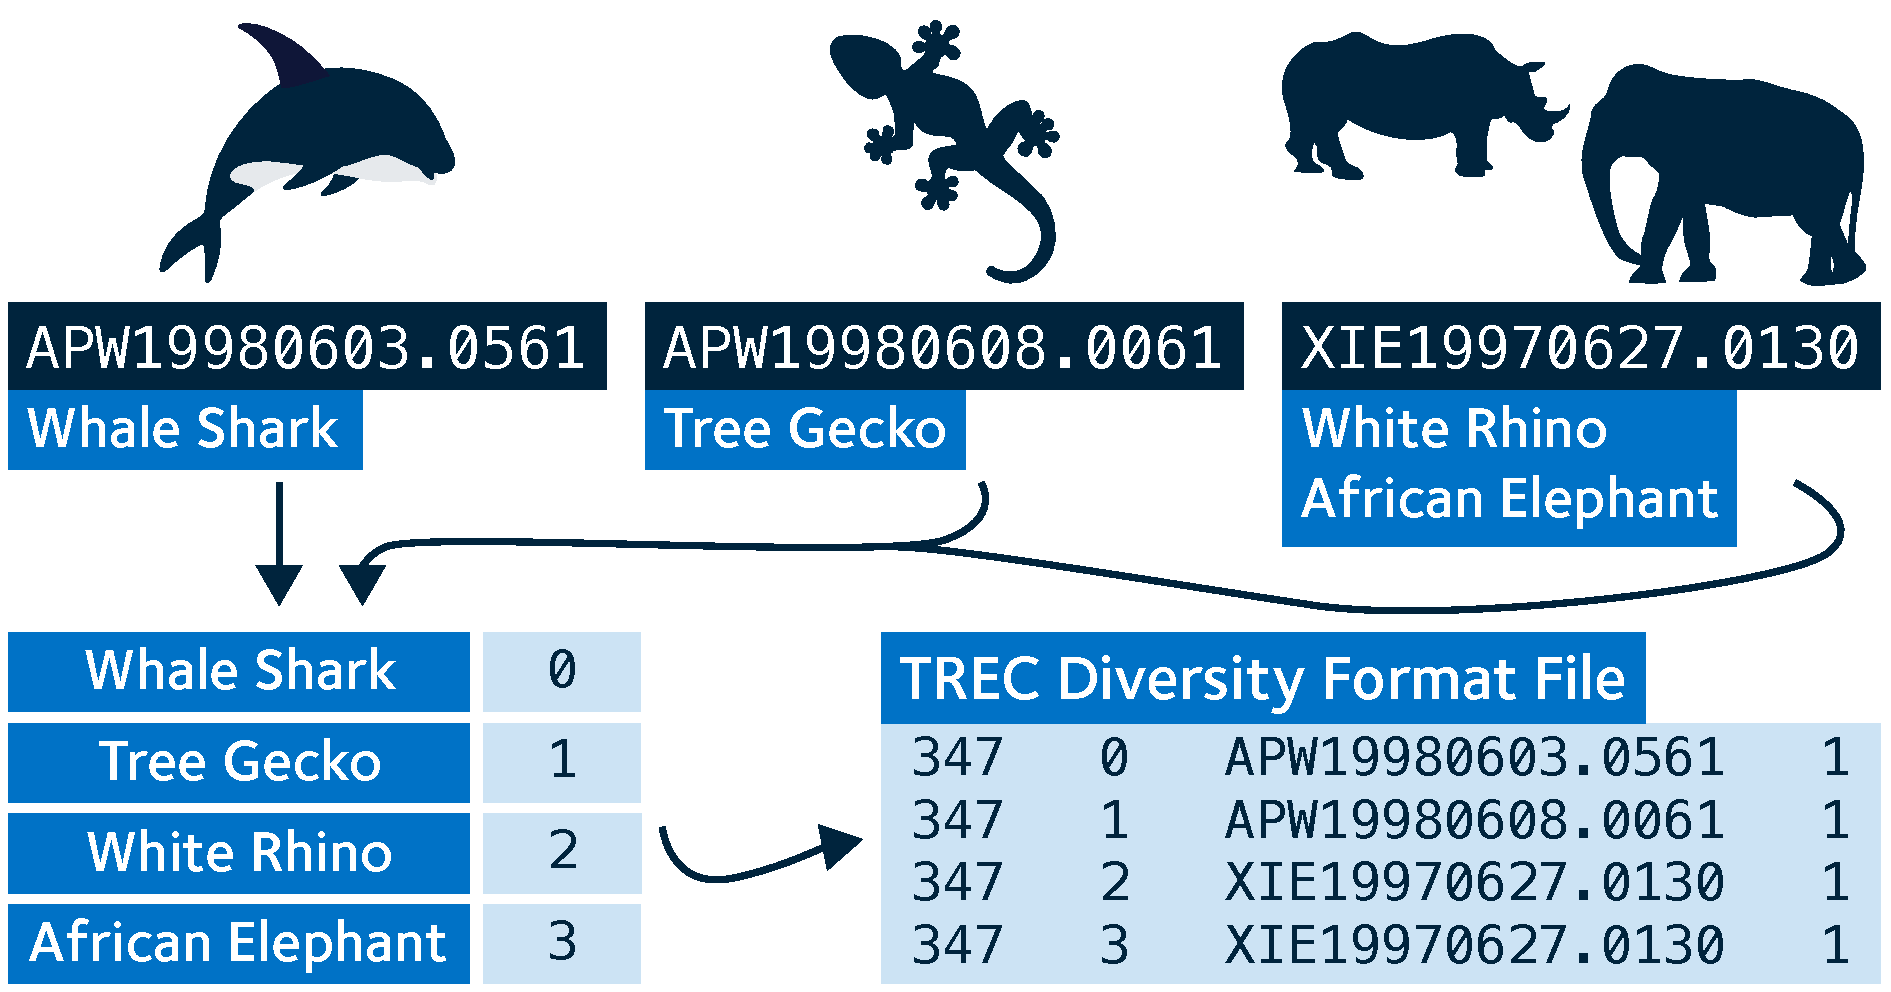
\includegraphics{figures/ch8-entity_ids.pdf}}
    \caption[Entity-based aspects example]{An example of documents, each with one or more entity-based aspects discussed within them. From these identified aspects, we can then provide a unique identifier for each aspect per topic, before creating a~\gls{acr:trec} diversity format file to be used in evaluation applications such as \texttt{ndeval}, allowing us to compute many diversity-based measures.}
    \label{fig:entity_ids}
\end{figure}

\subsubsection{Additional Performance Measures}\label{sec:diversity:users:measures}
In conjunction with the standard performance measures that we discussed back in Section~\ref{sec:csm:methodology:extracting:performance} on page~\pageref{sec:csm:methodology:extracting:performance}, we also include for this chapter two additional measures that consider aspectual search tasks. While traditional measures consider what documents are relevant, these additional measures allow us to determine \emph{why} said documents are relevant (i.e. what aspects each document covers).

The first measure we consider is \emph{aspectual recall (AR).} As part of the TREC-6 campaign,~\cite{over1998trec} defined aspectual recall as:

\begin{quote}
    \emph{``...the fraction of the submitted documents which contain one or more aspects.''}
    \attrib{\cite{over2001trec}}
\end{quote}

\begin{wrapfigure}[3]{r}{0.45\textwidth}
    \begin{center}
    \vspace*{-5mm}
    
\includegraphics[width=1\textwidth]{figures/ch8-aspectual_recall.pdf}
    \end{center}
    \vspace*{-4mm}
    \label{fig:aspectual_recall}
\end{wrapfigure}

Given a ranking, aspectual recall can be therefore computed by summing the number of \emph{unseen aspects} regarding a given topic up to a given ranking, $k$, and dividing by the rank. This is in contrast to more simplistic relevance measures, that consider only the~\gls{acr:trec} relevance judgement score for a document and topic combination. An example is provided above: given three documents, with three, one and zero new aspects to a topic, the aspectual recall at rank 3 is therefore $(3+1+0)/3 = 1.33$.

In addition to aspectual recall, \emph{aspectual precision} was also defined by~\cite{over2001trec} as \emph{``the fraction of total aspects...for the topic that are covered by the submitted documents.''} Given this definition, it was argued by~\cite{sanderson2010test} that aspectual precision appears to be the same as precision, and thus we do not report aspectual precision in this chapter.

The second measure that considers the diversity of the results returned is $\alpha DCG$. A~\glsfirst{acr:cg}-based approach, we discuss~\gls{acr:cg} basics in Section~\ref{sec:ir_background:user:evaluation:cg}. An extension of~\glsfirst{acr:dcg}~\citep{jarvelin2002cg}, $\alpha DCG$ employs a position-based user model~\citep{clarke2008adcg}. The measure takes into account the position at which a document is ranked along with the aspects contained in the documents. $\alpha DCG$ ranks by rewarding newly-found aspects, and penalising redundant aspects geometrically, discounting all rewards with a discounting rank function. As the name of the measure might imply, $\alpha$ is a tuneable parameter, controlling the severity of redundancy penalisation. As used in prior~\gls{acr:trec} experimentation, we used $\alpha=0.5$ for all reporting of $\alpha DCG$ in this chapter.
% Based on "Analysis of Various Evaluation Measures for Diversity" by Chandar

\subsubsection{Diversifying Search Results}\label{sec:diversity:users:diversifying}
As discussed earlier, our system factor considered both a baseline BM25 retrieval system, and a diversified approach, again using BM25 as an initial ranking baseline. The algorithm that we employed, based upon the \emph{XQuAD} framework by~\cite{santos2010query_reformulations_diversification}, re-scores and subsequently re-ranks documents based upon the number of unseen entities that appear within the document. The algorithm is presented as pseudo-code in Algorithm~\ref{alg:diversifying} below. Essentially, documents are re-ranked according to the number of new entities that are contained within them, with $w$ determining the weighting of the aspectual scoring component.

\renewcommand{\figurename}{Figure/Algorithm}
\begin{figure}[t!]
    \centering
    \resizebox{1\hsize}{!}{
    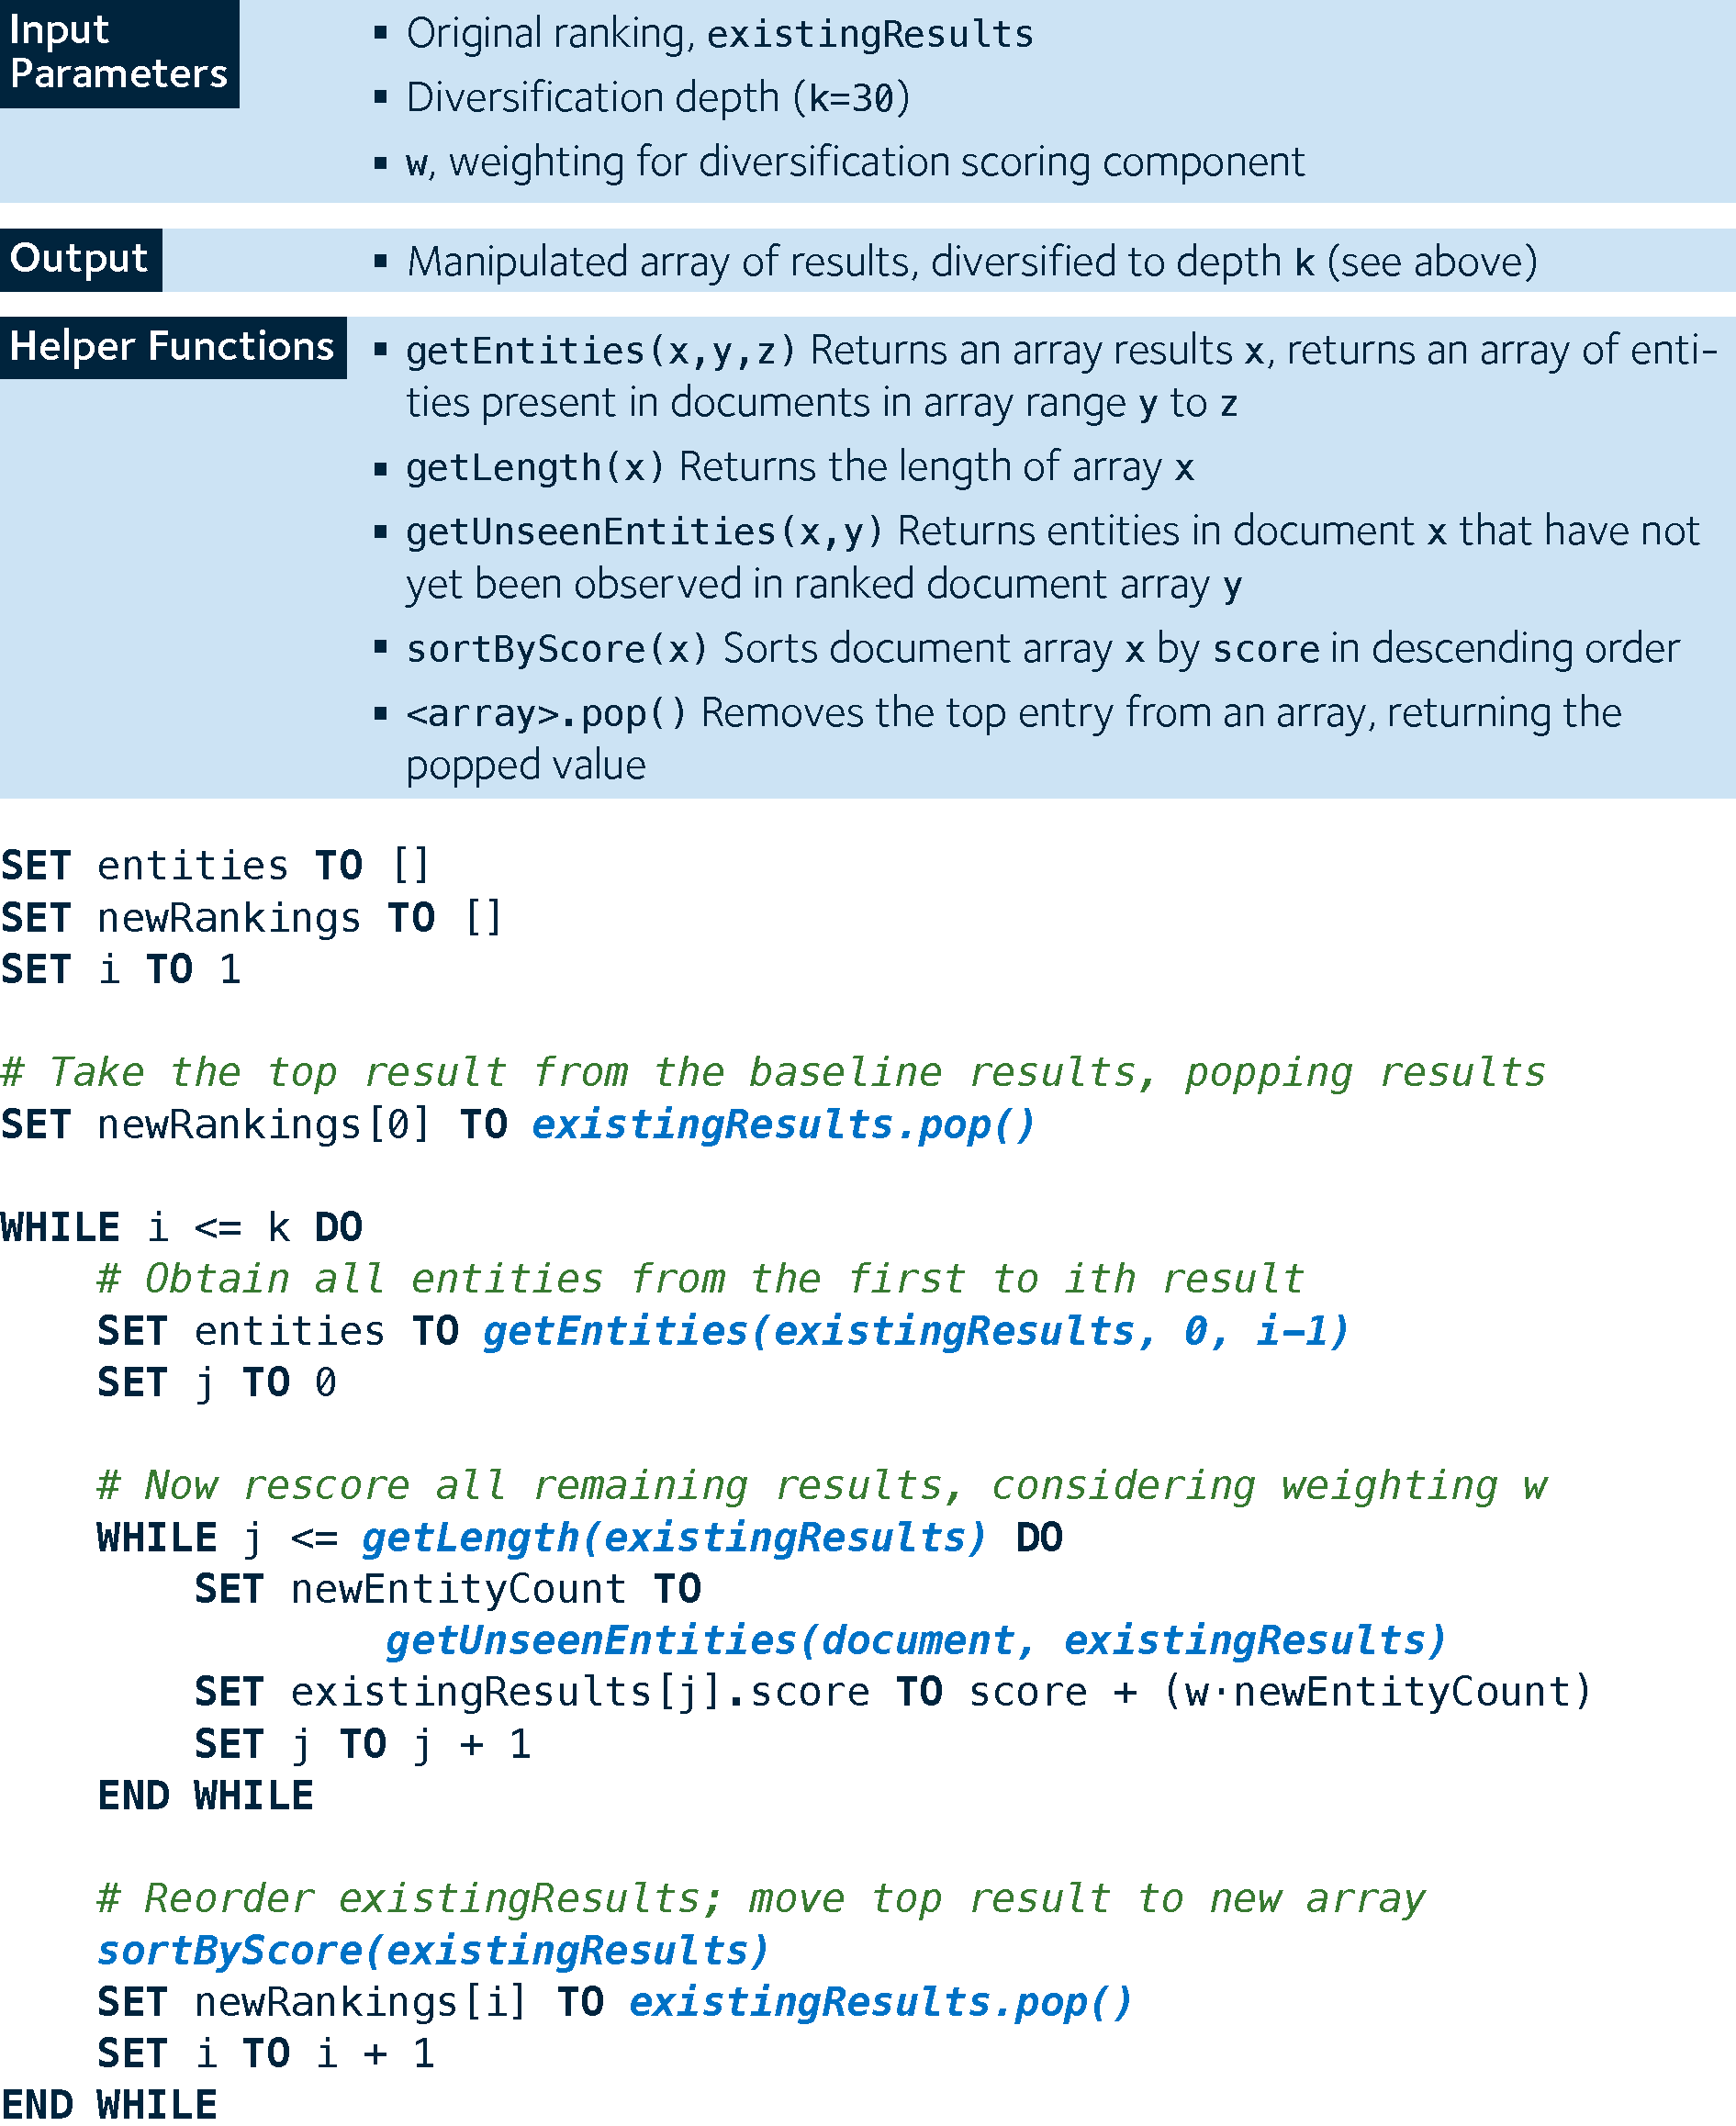
\includegraphics{figures/ch8-pseudocode.pdf}}
    \caption[Diversification algorithm pseudo-code]{Pseudo-code of the diversification algorithm used in this study, based upon the XQuAD framework by~\cite{santos2010query_reformulations_diversification}. As described in Section~\ref{sec:diversity:users:diversifying}, the algorithm guarantees that~\gls{acr:trec} relevant documents containing different aspects from each other will bubble up the baseline (BM25) rankings. Psuedo-code is provided in \emph{HAGGIS}~\citep{cutts2014haggis}.}
    \label{alg:diversifying}
\end{figure}
\renewcommand{\figurename}{Figure}

In order to select a reasonable approximation for the algorithm's $w$ weighting, we performed a pilot study, running the diversification algorithm over the set of $715$ queries that were issued by subjects of the user study reported in Chapter~\ref{chap:snippets}. Results of the pilot study are presented in Table~\ref{tbl:aspects_previous_queries}. As can be seen from the table, we explored a range of cutoff ($k$) and weighting ($w$) values, with $10-50$ trialled for $k$ and $0.1-1.0$ trialled for $w$. We selected $k=30, w=0.7$ as this combination provided the best results ($AR@10=6.61$, $\alpha DCG=0.075$, $P@10=0.36$) in terms of performance and efficiency. A higher $k$ for example only slightly increased performance, but took longer to compute. Indeed, $k=30$ was deemed to be a sensible choice as subjects from the prior user study didn't go lower than a depth of $24$ on average over interface \blueboxbold{T0}.

\begin{table}[t!]
    \caption[Aspectual recall pilot study results]{Table illustrating the effects of varying the diversification weighting parameter, \emph{w}, and diversification cutoff \emph{k} when using the diversification algorithm as discussed in Section~\ref{sec:diversity:users:diversifying}. Value in the table represent the aspectual recall in the top 10 documents after re-ranking, on average, over the 715 queries issued by subjects of the user study reported in Chapter~\ref{chap:snippets}. At \emph{w=0.0}, diversification is not applied – this configuration therefore enjoys the same performance as our baseline, non-diversified system \blueboxbold{ND}, utilising BM25 \emph{(b=0.75).}\vspace*{-3mm}}
    \label{tbl:aspects_previous_queries}
    \renewcommand{\arraystretch}{1.8}
    \begin{center}
    \begin{tabulary}{\textwidth}{L{0.4cm}@{\CS}D{2cm}@{\CS}D{2.12cm}@{\CS}D{2.12cm}@{\CS}D{2.12cm}@{\CS}D{2.12cm}@{\CS}D{2.12cm}@{\CS}}
    
    \RS & & \multicolumn{5}{c}{\hspace*{-5mm}\textbf{Cutoff Range (k)}}\\
    
    \RS & & \lbluecell\textbf{10} & \lbluecell\textbf{20} & \lbluecell\textbf{30} & \lbluecell\textbf{40} & \lbluecell\textbf{50}\\
    
    \RS \multirow{7}{*}{\rotatebox{90}{\hspace*{-10mm}\textbf{Weighting Parameter}}} & \lbluecell\textbf{0.0 (ND)} & \multicolumn{5}{@{\hskip 0pt}c@{\CS}}{\cell \textbf{3.64}} \\
    
    \RS & \lbluecell\textbf{0.1} & \cell 3.64 & \cell 4.94 & \cell 5.51 & \cell 5.95 & \cell 6.37 \\
    \RS & \lbluecell\textbf{0.3} & \cell 6.58 & \cell 6.58 & \cell 6.64 & \cell 6.59 & \cell 6.59 \\
    \RS & \lbluecell\textbf{0.5} & \cell 6.58 & \cell 6.58 & \cell 6.58 & \cell 5.58 & \cell 6.58 \\
    \RS & \lbluecell\textbf{0.7 (D)} & \cell 6.56 & \cell 6.56 & \cell \textbf{6.61} & \cell 6.51 & \cell 6.60 \\
    \RS & \lbluecell\textbf{0.9} & \cell 6.52 & \cell 6.52 & \cell 6.61 & \cell 6.57 & \cell 6.63 \\
    \RS & \lbluecell\textbf{1.0} & \cell 6.63 & \cell 6.63 & \cell 6.59 & \cell 6.61 & \cell 6.56 \\
    
\end{tabulary}
\end{center}
\end{table}

For the diversity re-ranking to work in this scenario, the algorithm must be aware of the ground truths which were collated, as described in Section~\ref{sec:diversity:users:method:aspects} above. The reasons for following this approach were:

\begin{itemize}
    \item{us not having to invest a significant amount of effort tuning a different diversification algorithm to return acceptable results; and}
    \item{that it would guarantee that~\gls{acr:trec} relevant documents, containing different entities, would bubble up to the top of the rankings, increasing the effect (and hopefully subject observation) that the results were indeed ranked differently.}
\end{itemize}

Without such a ground truth based approach, ensuring that~\gls{acr:trec} relevant documents would bubble up would have been difficult to achieve. Given the effects of document pooling as part of how the~\gls{acr:trec} QRELs were created (refer to Section~\ref{sec:ir_background:basics:cranfield}), it is highly likely that many other documents exist within the corpus that could be considered to be useful to a given topic, but were not assessed.

\blueboxheader{Avoiding Perfect Results}
As previously discussed, one major pitfall of this approach is that the diversification algorithm would have become \emph{too perfect.} With access to the ground truths, it would subsequently proceed to assign a higher rank to documents that were~\gls{acr:trec} assessed, leading to every document in the top $k$ containing new entities. To make this more of a challenge for subjects, we also incorporated within our aspectual data documents that were considered to be non-relevant by~\gls{acr:trec} assessors (i.e. a~\gls{acr:trec} assessment of $0$). This led to including an additional $2,663$ document that would be included within the diversity re-ranking, but were not relevant. For each of the five topics we consider in this thesis, the number of non-relevant documents from the~\gls{acr:trec} QRELs over each topic were:

\begin{itemize}
    \item{\blueboxbold{Airport Security} with 580 non-relevant documents;}
    \item{\blueboxbold{Wildlife Extinction} with 500 non-relevant documents;}
    \item{\blueboxbold{Piracy} with 526 non-relevant documents;}
    \item{\blueboxbold{Tropical Storms} with 502 non-relevant documents; and}
    \item{\blueboxbold{Curbing Population Growth} with 555 non-relevant documents.}
\end{itemize}

Rather than manually assess each document, we took the list of entities that were discovered for~\gls{acr:trec} relevant documents, and performed an exact keyword search for each of the entities within each of the $2,663$ documents. Any matches would have the corresponding entity attached to the document.

\subsubsection{Post-Task Surveys}
With the pre-task survey the same as that outlined in the general methodology (refer to Section~\ref{sec:csm:methodology:extracting:user}), surveys for this study differed post-task and post-experiment. Here, we discuss the questions posed in each of the four post-task surveys.

On the completion of each of the four search tasks, subjects were asked to answers questions that were split into two broad categories, examining:

\begin{itemize}
    \item{their perceived behaviours when interacting; and}
    \item{how they felt the retrieval system they used had performed.}
\end{itemize}

Answers were compulsory; we provided a seven-point Likert scale for responses, providing the ability to give a neutral response, as well as strong agreement or disagreement with the questions that were posed.

Considering the subject's behaviours, we asked their opinions on the following areas.

\begin{itemize}
    \item{\blueboxbold{Success} How successful they thought they were at completing the given search task.}
    \item{\blueboxbold{Subject Speed} How quickly subjects felt that they completed the search task.}
    \item{\blueboxbold{Queries} Whether the subjects issued different queries to explore the topic.}
    \item{\blueboxbold{Documents} If they only examined a small number of documents per query.}
    \item{\blueboxbold{Checks} Whether they checked each document carefully before saving.}
    \item{\blueboxbold{Enough} Whether the subjects saved more documents than was required (remembering that subjects were instructed to save a minimum of four per task).}
\end{itemize}

In addition to the behavioural component of the survey, the system-sided component of the survey asked an additional six questions, again using a seven-point Likert scale. The questions posed to the subjects are enumerated below.

\begin{itemize}
    \item{\blueboxbold{System Speed} How well subjects thought the system helped them complete the given search task quickly.}
    \item{\blueboxbold{Difficulty} Whether they felt the system made things difficult to find useful information.}
    \item{\blueboxbold{Ease} If the system made it easy for subjects to complete the given search task.}
    \item{\blueboxbold{Happiness} Whether the subjects were happy or not with how the system performed.}
    \item{\blueboxbold{Cumbersome} Whether they felt the system was cumbersome to use or not.}
    \item{\blueboxbold{Confidence} How confident the subjects were in the decisions that they had taken.}
\end{itemize}

\subsubsection{Post-Experiment Survey}
In addition to the post-task surveys, we also asked subjects to answer a post-experiment survey upon completion of all four search tasks. Here, we wanted to ascertain which of the two retrieval systems (Hula Search, representing the baseline, non-diversified system \blueboxbold{ND} or YoYo Search, representing the diversified system, \blueboxbold{D}) offered subjects a better experience, and which one of the two that they preferred overall.

Seven questions were posed, with answers again provided on a Likert scale. However, we this time provided six possible choices, from $1$ (definitely Hula Search) to $3$ (slightly Hula Search), from $4$ (slightly YoYo Search) to $6$ (definitely YoYo Search). We opted not to include a neutral option to force subjects into deciding between one of the two systems. We asked the subjects the following questions.

\begin{itemize}
    \item{\blueboxbold{Informative} Of the two retrieval systems, subjects were asked to pick which of the two returned the most informative results.}
    \item{\blueboxbold{Unhelpful} What one of the two retrieval systems was the most unhelpful?}
    \item{\blueboxbold{Easiest} Of the two retrieval systems, what one was the easiest to use?}
    \item{\blueboxbold{Least Useful} Which retrieval system was the least useful?}
\end{itemize}

The final three questions then led on to asking subjects about what one of the two systems they felt yielded the most relevant and diverse content.

\begin{itemize}
    \item{\blueboxbold{Most Relevant} Which of the two retrieval systems yielded the most relevant information?}
    \item{\blueboxbold{Most Diverse} Which of the two retrieval systems offered the more diverse set of results?}
    \item{\blueboxbold{Most Preferable} Which retrieval system did you prefer overall?}
\end{itemize}

While responses from subjects did definitely provide a preferred retrieval system, we nevertheless discuss the results from this survey in Section~\ref{sec:diversity:users:results:experience}.

\subsection{Results}

\subsubsection{Interactions}

\subsubsection{Time-Based}

\subsubsection{Performance}

\subsubsection{User Experience}\label{sec:diversity:users:results:experience}

\subsubsection{Gain over Time}

\subsection{Discussion}

\section{Simulated Analysis}\label{sec:diversity:simulated}

\section{Chapter Summary}